\newpage
\appendix
\onecolumn

\section{Definitions}

\subsection{Self-Supervision}
Self-supervision is a learning paradigm in which a model is trained using automatically generated labels rather than human-annotated data. This technique is commonly used to leverage large amounts of unlabeled data by designing tasks that encourage the model to learn meaningful representations.

\section{Backbone Networks}

\subsection*{YOLO}
YOLO, developed by Ultralytics, is a CNN-based model capable of detecting 17 key points of a person in a frame. It is widely used for pose estimation and action recognition.

\subsection*{R3D}
ResNet-3D (R3D) is a 3D CNN architecture proposed in \cite{resnet-3d} for video classification. It extends the original ResNet architecture to process spatio-temporal data.

\subsection*{I3D}
Inflated 3D (I3D) is a 3D CNN network proposed in \cite{i3d} for video classification. It extends the Inception architecture to 3D by inflating 2D convolutional filters into 3D filters. The model initializes its weights using pretrained 2D CNN models to improve convergence and performance. I3D employs a two-stream approach that processes optical flow and RGB frames separately through dedicated 3D CNNs, merging the outputs for classification.

\subsection*{DINO}
DINO, introduced in \cite{dinov2}, is a transformer-based vision model pre-trained on a large image dataset. It leverages a class token, whose state in the final layer serves as the feature representation. DINO demonstrates strong generalization capabilities on various visual tasks.

\subsection*{CLIP}
CLIP is a vision transformer model designed for zero-shot learning. Trained on extensive image-text pairs, CLIP effectively classifies images based on text descriptions and vice versa.

\subsection*{X3D}
X3D, proposed in \cite{x3d}, is an efficient and lightweight family of 3D CNNs designed for video understanding. By expanding a 2D CNN across multiple axes, X3D reduces parameters and computations while maintaining strong performance.

\subsection*{S3D}
S3D, described in \cite{s3d}, is a 3D CNN architecture designed for video-text embeddings. The model replaces certain 3D convolution steps with 2D convolutions equipped with temporal kernels. This modification improves efficiency and facilitates training on large-scale instructional video datasets.

\subsection*{SlowFast}
SlowFast, introduced in \cite{slowfast}, is a two-stream network that processes video at two different frame rates. The slow path captures spatial semantics and high-level features, while the fast path captures rapid motion dynamics at a higher temporal resolution.

\subsection*{ViViT}
ViViT, proposed in \cite{vivit}, extends the vision transformer architecture to video data. Each video frame is processed by a vision transformer, extracting CLS tokens that are then combined using a second transformer to capture temporal relationships and produce a final video embedding.

\newpage
\section{Figures and Tables}

\begin{table}[!h]
    \centering
    \small
    \resizebox{1\linewidth}{!}{
    \begin{tabular}{lcrrr}
    \toprule
    Backbone & Type & $\#$Parameters & $\#$Frames & Features Shape \\
    \midrule
    yolo & By Frame & 2.9M & 8 & (8, 34) \\
    dino & By Frame & 22.1M & 8 & (8, 384) \\
    clip & By Frame & 151.3M & 8 & (8, 512) \\
    r3d & By Segment & 31.6M & 8 & (2048, 1) \\
    i3d & By Segment & 12.7M & 16 & (1024, 1) \\
    x3d-xs & By Segment & 3.0M & 4 & (2048, 1) \\
    x3d-s & By Segment & 3.0M & 16 & (2048, 1) \\
    x3d-m & By Segment & 3.0M & 16 & (2048, 1) \\
    x3d-l & By Segment & 5.3M & 16 & (2048, 1) \\
    s3d-k & By Segment & 7.9M & 16 & (1024, 1) \\
    s3d-h & By Segment & 9.7M & 16 & (1024, 1) \\
    slowfast & By Segment & 33.6M & 32 & (2304, 1) \\
    vivit & By Segment & 88.6M & 32 & (768, 1) \\
    \bottomrule
    \end{tabular}
    }
    \vspace{-2ex}\caption{Detailed Descriptions of Feature Extractors.}
    \end{table}

\begin{figure}[!h]
    \centering
    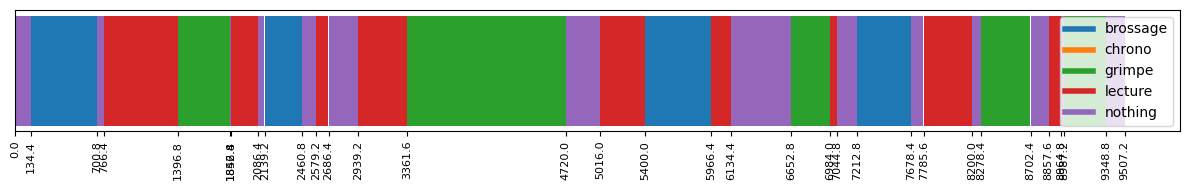
\includegraphics[width=\textwidth]{../../assets/figures/example-of-video-segmentation-1.png}
    \caption{Example of video segmentation generated using the TAS helper Python package.}
    \label{fig:your-label}
\end{figure}